\chapter{Preliminaries}

The field of autonomous driving agents has rapidly increased in modern car manufacturing. Current research topic rises the agents from parking or lane keeping assistant fully autonomous driving agents obeying the traffic rules and having the ability to react to the volatile environment in a reasonable way.

For that machine learning techniques have proven themselves as an essential part. But in order to fulfil the security standards and create a sophisticated agent it has to be trained on hundred-thousands of scenarios each having a large set of data attached, for example sensor and camera data.
The approach of \textit{Convolutional Neural Networks} (CNNs) have been proven to be powerful enough to handle such many training iterations with a huge number of input variables, while maintaining the large learning capacity. \cite{krizhevsky2012imagenet}

A CNN, as explained in \Cref{sec:CNN}, has a general structure, but can be altered to fit into the approach in various ways influencing the result. Therefore we introduce in \Cref{sec: Deep Learning Approaches} the three main approaches of using a CNN.

Further in \Cref{chapter: DLL} we see that there is the need of specific languages for the design and implementation of such agents. Two languages will be discussed and compared based on their suitability regarding the \alexnet, stated in  \Cref{sec: AlexNet}.

\section{Neural Networks}\label{sec: NN}

The \nns are a construct adapted from biological processes. The general construct is very simple, but the expressiveness is very high but still not fully researched.
A neural net is made out of neurons and has one very basic function:
It takes a fixed number $n \in \mathbb{N}$ of the incoming values $x_i$, where the vector $(x_0,\dots x_n)^T$ is called a tensor, and multiplies them each with a specific weight $w_i$, where $0 \le i \le n$.
Also every neuron contains a bias $b$, which is a general value subtracted from the sum, so $\sum_{i=0}^{n} (x_i \cdot w_i) -b$. 

Often one applies an activation function to fix the value between 0 and 1. Such a function would be for example the sigmoid function or the ReLu, which are both non-linear functions. Without using a non-linear one gets restricted to linear regression and therefore reducing the ability to model more complex functions.
This non-linear normalized value gets forwarded to the neurons of the next layer.

Those neurons are ordered in different groups often called layers, as seen in \Cref{fig: Simple NN}.
\begin{enumerate}
	\item input layer (green):\\ \label{item input layer}
	This layer gets fed with the input values of the problem, which can be for example sensor data or pixel color values.
	\item hidden layer (blue):\\\label{item hidden layer}
	The hidden layer consists of neurons receiving the values from the previous layer, while not being obliged to have the same number of neurons (c.f. \Cref{fig: Simple NN}).
	Different hidden layer architectures can be distinguished to be deep (c.f. \Cref{fig: Deep Neural Net}). This means, that there are multiple layers of neurons within the hidden layer itself.\\
	Also a variation within the hidden layer is the possibility of fully connectivity (c.f. \Cref{fig: not fullyconnected Neural Net}). Thus some neurons don't forward their value to every neuron of the next layer.\\
	There is no rule of how to construct the best hidden layer, considering number of sub-layers, neurons per layer or the connectivity.
	\item output layer (yellow):\label{item output layer}
	The output neurons contain the value the \nn produces. Depending on the \nns purpose it can be for example a confidence value of a classification, like recognizing a stop sign, or the value of changing the steering wheel angle. 
\end{enumerate}

In order to train a \nn one has to define the behaviour the \nn should have. In an image classification example one should know what the correct class of a given image of a sign is, i.e. a speed limit sign.\\
A \nn can then be trained by giving it values for the input layer and comparing the values of the output layer with the solutions it should have resulted in. The difference can then be checked. Such a difference can be simply \texttt{true}/\texttt{false} or a value indicating how big the difference is. In the example of signs a classification of a ``speed limit 70''-sign as ``speed limit 50''-sign is still wrong, but as bad as a classification as a ``stop''-sign.\\
Using this difference value the \nn can use linear algebra algorithms to adjust the weights $w_i$ and biases $b$ to improve the output iteratively.

Further information about the underlying training algorithms like gradient descend, newtons method, conjugate gradient or Levenberg-Marquardt algorithm is not given here in order to keep the paper in a justifiable length.  

\begin{figure}
	\centering
	\tikzset{input/.style = {ellipse,draw,fill=green!50!white, initial, initial text =}}
	\tikzset{hidden/.style = {ellipse,draw,fill=blue!50!white}}
	\tikzset{output/.style = {ellipse,draw,fill=yellow!50!white}}
	\begin{subfigure}[b]{0.25\textwidth}
	\begin{tikzpicture}[node distance = .5cm, on grid,auto]		
		\node[input] (i1) {};
		\node[input, below = of i1] (i2) {};
		\node[input, below = of i2] (i3) {};
		
		\node[hidden, above right = .25cm and 1cm of i1] (h1) {};
		\node[hidden, below = of h1] (h2) {};
		\node[hidden, below = of h2] (h3) {};
		\node[hidden, below = of h3] (h4) {};
		
		\node[output , right = 1cm of h2] (o1) {};
		\node[output , below = of o1] (o2) {};
		\coordinate[right = of o1] (c1) {};
		\coordinate[right = of o2] (c2) {};
		
		\path[->] (i1.east) edge (h1.west)
					(i1.east) edge (h2.west)
					(i1.east) edge (h3.west)
					(i1.east) edge (h4.west);
		\path[->] (i2.east) edge (h1.west)
					(i2.east) edge (h2.west)
					(i2.east) edge (h3.west)
					(i2.east) edge (h4.west);
		\path[->] (i3.east) edge (h1.west)
					(i3.east) edge (h2.west)
					(i3.east) edge (h3.west)
					(i3.east) edge (h4.west);
		\path[->] (h1.east) edge (o1.west)
				  (h2.east) edge (o1.west)
				  (h3.east) edge (o1.west)
				  (h4.east) edge (o1.west);
		\path[->] (h1.east) edge (o2.west)
					(h2.east) edge (o2.west)
					(h3.east) edge (o2.west)
					(h4.east) edge (o2.west);
		\path[->] (o1) edge (c1)
				  (o2) edge (c2);		
	\end{tikzpicture}	
	\caption{}
	\label{fig: Simple NN}
	\end{subfigure}
	\begin{subfigure}[b]{0.40\textwidth}
	\begin{tikzpicture}[node distance = .5cm, on grid,auto]		
	\node[input] (i1) {};
	\node[input, below = of i1] (i2) {};
	\node[input, below = of i2] (i3) {};
	
	\node[hidden, above right = .25cm and 1cm of i1] (h11) {};
	\node[hidden, below = of h11] (h21) {};
	\node[hidden, below = of h21] (h31) {};
	\node[hidden, below = of h31] (h41) {};
	
	\node[hidden, above right = .5cm and 1cm of h11] (h12) {};
	\node[hidden, below = of h12] (h22) {};
	\node[hidden, below = of h22] (h32) {};
	\node[hidden, below = of h32] (h42) {};
	\node[hidden, below = of h42] (h52) {};
	\node[hidden, below = of h52] (h62) {};
	
	\node[right =0.5cm of h12] (d1) {\dots};
	\node[below = of d1] (d2) {\dots};
	\node[below = of d2] (d3) {\dots};
	\node[below = of d3] (d4) {\dots};
	\node[below = of d4] (d5) {\dots};
	\node[below = of d5] (d6) {\dots};
	
	\node[hidden, right = 0.5cm of d1] (h13) {};
	\node[hidden, below = of h13] (h23) {};
	\node[hidden, below = of h23] (h33) {};
	\node[hidden, below = of h33] (h43) {};
	\node[hidden, below = of h43] (h53) {};
	\node[hidden, below = of h53] (h63) {};
	
	\node[output , right = 1cm of h33] (o1) {};
	\node[output , below = of o1] (o2) {};
	\coordinate[right = of o2] (c1) {};
	\coordinate[right = of o1] (c1) {};
	
	\path[->] (i1.east) edge (h11.west)
				(i1.east) edge (h21.west)
				(i1.east) edge (h31.west)
				(i1.east) edge (h41.west);
	\path[->] (i2.east) edge (h11.west)
				(i2.east) edge (h21.west)
				(i2.east) edge (h31.west)
				(i2.east) edge (h41.west);
	\path[->] (i3.east) edge (h11.west)
				(i3.east) edge (h21.west)
				(i3.east) edge (h31.west)
				(i3.east) edge (h41.west);
	\path[->] (h11.east) edge (h12.west)			
				(h11.east) edge (h22.west)
				(h11.east) edge (h32.west)
				(h11.east) edge (h42.west)
				(h11.east) edge (h52.west)
				(h11.east) edge (h62.west);
	\path[->] (h21.east) edge (h12.west)			
				(h21.east) edge (h22.west)
				(h21.east) edge (h32.west)
				(h21.east) edge (h42.west)
				(h21.east) edge (h52.west)
				(h21.east) edge (h62.west);
	\path[->] (h31.east) edge (h12.west)			
				(h31.east) edge (h22.west)
				(h31.east) edge (h32.west)
				(h31.east) edge (h42.west)
				(h31.east) edge (h52.west)
				(h31.east) edge (h62.west);			
	\path[->] (h41.east) edge (h12.west)			
				(h41.east) edge (h22.west)
				(h41.east) edge (h32.west)
				(h41.east) edge (h42.west)
				(h41.east) edge (h52.west)
				(h41.east) edge (h62.west);
					
	\path[->] (h13.east) edge (o1.west)
				(h23.east) edge (o1.west)
				(h33.east) edge (o1.west)
				(h43.east) edge (o1.west)
				(h53.east) edge (o1.west)
				(h63.east) edge (o1.west);		
	\path[->] (h13.east) edge (o2.west)
				(h23.east) edge (o2.west)
				(h33.east) edge (o2.west)
				(h43.east) edge (o2.west)
				(h53.east) edge (o2.west)
				(h63.east) edge (o2.west);		
	\end{tikzpicture}
	\caption{}
	\label{fig: Deep Neural Net}
	\end{subfigure}	
	\begin{subfigure}[b]{0.32\textwidth}
		\begin{tikzpicture}[node distance = .5cm, on grid,auto]		
		\node[input] (i1) {};
		\node[input, below = of i1] (i2) {};
		\node[input, below = of i2] (i3) {};
		
		\node[hidden, above right = .25cm and 1cm of i1] (h11) {};
		\node[hidden, below = of h11] (h21) {};
		\node[hidden, below = of h21] (h31) {};
		\node[hidden, below = of h31] (h41) {};
		
		\node[hidden, above right = .5cm and 1cm of h11] (h12) {};
		\node[hidden, below = of h12] (h22) {};
		\node[hidden, below = of h22] (h32) {};
		\node[hidden, below = of h32] (h42) {};
		\node[hidden, below = of h42] (h52) {};
		\node[hidden, below = of h52] (h62) {};
		
		
		\node[output , right = 1cm of h32] (o1) {};
		\node[output , below = of o1] (o2) {};
		\coordinate[right = of o2] (c1) {};
		\coordinate[right = of o1] (c1) {};
		
		\path[->] (i1.east) edge (h11.west)
			(i1.east) edge (h21.west)
			(i1.east) edge (h31.west)
			(i1.east) edge (h41.west);
		\path[->] (i2.east) edge (h11.west)
			(i2.east) edge (h21.west)
			(i2.east) edge (h31.west)
			(i2.east) edge (h41.west);
		\path[->] (i3.east) edge (h11.west)
			(i3.east) edge (h21.west)
			(i3.east) edge (h41.west);

		\path[->] (h11.east) edge (h12.west)			
			(h11.east) edge (h22.west)
			(h11.east) edge (h32.west);
		\path[->] (h21.east) edge (h22.west)
			(h21.east) edge (h32.west)
			(h21.east) edge (h42.west)
			(h21.east) edge (h12.west);
		\path[->] (h31.east) edge (h32.west)
			(h31.east) edge (h42.west)
			(h31.east) edge (h52.west)
			(h31.east) edge (h62.west);			
		\path[->] (h41.east) edge (h42.west)
			(h41.east) edge (h52.west)
			(h41.east) edge (h62.west);
		\path[->] (h12.east) edge (o1.west)
			(h22.east) edge (o1.west)
			(h52.east) edge (o1.west)
			(h62.east) edge (o1.west);		
		\path[->] (h12.east) edge (o2.west)
			(h22.east) edge (o2.west)
			(h32.east) edge (o2.west)
			(h42.east) edge (o2.west)
			(h52.east) edge (o2.west)
			(h62.east) edge (o2.west);		
		\end{tikzpicture}
		\caption{}
		\label{fig: not fullyconnected Neural Net}
	\end{subfigure}
	% das Dritte ist wenig Sinvoll vom Aufbau her
\end{figure}


\section{Convolutional Neural Network (CNN)}\label{sec:CNN}

A CNN is a special class of deep feed-forward \nns. On of the main design goals of a CNN is that they require a minimal amount of preprocessing. This is an important aspect, because they are often fed with images. Preprocessing high resolution images is very costly in terms of computational time. In the context of autonomous driving the time is even more crucial, since the driving agent needs to be able to react to spontaneous events.

Like most parts of \nns, also the CNNs are inspired by biological processes. It is mainly based on the connectivity pattern of an animals visual cortex, where special neurons respond only to stimuli of their receptive field, represented as rectangles lying in the image. Partially overlapping guarantees a complete coverage of the field of view. Those rectangles are often called kernel or filters.\cite{matsugu2003subject}

%The partitioning into those rectangles can also have the advantage, that the size of the input image is not relevant. If there would be a direct correspondence of a pixel to one input value then a change of the size would infer null values or additional input values, where the weights are not directly well suited. But with partitioning it into sub-rectangles of the image the values can be unified by selecting these rectangles relative to the size.
%This is only given, if there are no fully connected layers. Otherwise one has to perform other steps like cropping, scaling or padding. %TODO ref

Using the so called pooling the net reduces the amount of inputs by mapping a number of values, for example the color values of a kernel, to one single value. One often used pooling type is the max pooling, which takes the maximal value of a property. Using pooling and relative sizes of kernels one can avoid the necessity of equally sized images. \cite{wiki:CNN} 

These separation into those receptive fields has also the advantage that is reduces the effort to train a CNN. The weights and biases of neurons of each receptive field are equal. This is reasonable since for example a speed limit road sign should be identified independent whether it is located next to the road, like on a normal road, or above the road, like on an highway. \cite{lecun2015lenet}

Further CNNs make strong and mostly correct assumptions about the nature of images, like stationary of statistics and locality of pixel dependencies. This leads to fewer connections and parameters, compared to a normal feed-forward neural net with similar sized layers, and therefore reduces the time it takes to be trained, while being only slightly worse in their best-performance. \cite{krizhevsky2012imagenet}


\section{AlexNet} \label{sec: AlexNet}

The \textit{\alexnet} is one of the best performing CNN architectures currently known. It is trained on the ImageNet subsets of \texttt{ILSVRC-2010} and \texttt{ILSVRC-2012}\footnote{Further information: http://www.image-net.org/challenges/LSVRC/} and became famous because of its result being way ahead of all other competitors.

A highly optimized GPU implementation of this architecture combined with innovative features is publicly available. Those features lead to improve performance and reduce training time.\cite{krizhevsky2012imagenet}

An important note is that the original test is dated back to 2012 and therefore was used with an overall GPU memory of 6 GB, with which training took abound six days. With modern hardware like new GPUs, SLI usage or even clusters, the training can be done faster, or the model can be trained with more data to improve performance. The improvement cased only by hardware can be roughly grasped through \cite{sze2017hardware}.

%\todo{maybe calc the possible speed up based on ``Hardware for Machine Learning''}

\begin{figure}[ht]
	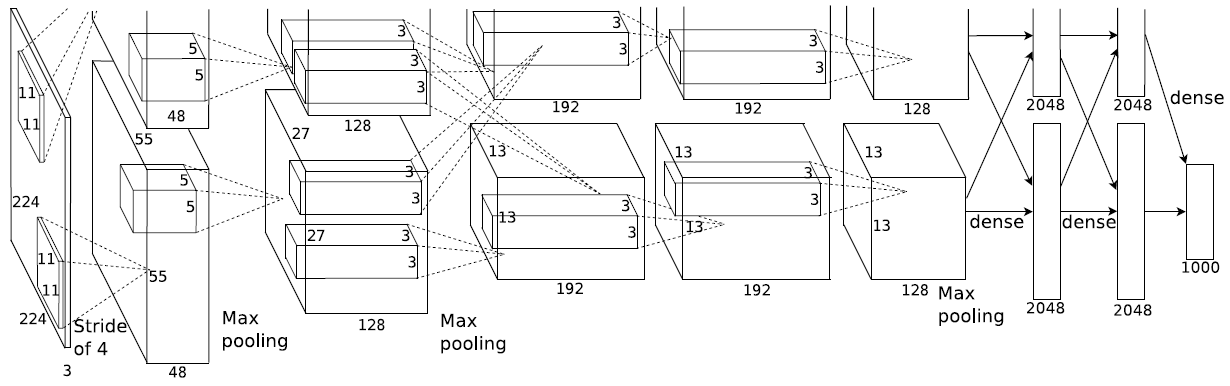
\includegraphics[scale = 0.5]{src/pic/AlexNet-structure.PNG}
	\caption{The \alexnet-architecture for two GPUs. It consists of 5 convolutional layers (at the beginning) and three fully-connected layers (at the end). The possibly multiple GPUs only communicate between two layers, but never within a layer.\cite{krizhevsky2012imagenet}}
	\label{pic: AlexNet}
	%TODO
%	\todo{Vereinfachen der Zeichnung\\}
\end{figure}